\section{Developing the simplex method}

In Chapter \ref{chapter_3}, we discussed all the necessary theoretical aspects required for the development of the simplex method. In this chapter, we will concentrate on operationalising the method under a computational standpoint.

\subsection{Calculating step sizes}

One discussion that we purposely delayed was that of how to define the value of the step size $\theta$ taken in the feasible direction $d$. Let $c \in \reals^n$, $A$ be a $m \times n$ full-rank matrix, $b$ a nonnegative $m$-sized vector (notice that this can be assumed without loss of generality, by a trivial transformation that does not change the constraint) and $J = \braces{1,\dots,n}$. Consider the linear programming problem $P$ in the standard form 
%
	\begin{equation*}
		(P) : \mini\braces{c^\top x : Ax = b, x \geq 0}.
	\end{equation*}
%
Building upon the elements we defined in Chapter \ref{chapter_3}, employing the simplex method to solve $P$ comprise the following set of steps:
%
\begin{enumerate}
	\item Start from a nondegenerate basic feasible solution (BFS)
	\item Find a negative reduced cost component $\overline{c}_j$. If $\overline{c} \geq 0$, return the current solution. 
	\item Move along the feasible direction $d = (d_B, d_N)$, where $d_j = 1$, $d_{N \setminus \braces{j}} = 0$ and $d_B = -B^{-1}A_j$.
\end{enumerate}
%
Moving along the feasible direction $d$ towards $x + \theta d$ (with $\theta > 0$) makes $x_j >0$ (i.e., $j \in I_N$ enter the basis), while reducing the objective value at a rate of $\overline{c}_j$. Thus, one should move as furthest as possible (say, $\overline{\theta}$) along the direction $d$, which incurs on an objective value change of $\overline{\theta} (c^\top d) = \overline{\theta} \overline{c}_j$.

Moving as far along the feasible direction $d$ as possible while observing that feasibility is retained is equivalent to setting $\overline{\theta}$ as 	
%
\begin{equation*}
	\overline{\theta} = \max\braces{\theta \geq 0 : A(x + \overline{\theta} d) = b, \ x + \overline{\theta}d \geq 0}.	
\end{equation*}
%
Recall that, by construction of the feasible direction $d$, we have that $Ad = 0$ and thus $A(x + \overline{\theta} d) = Ax = b$. Therefore, the only feasibility condition that can be violated when setting $\overline{\theta}$ too large is the nonnegativity of all variables, i.e., $x + \overline{\theta}d \geq 0$. 

To avoid this to be the case, all basic variables $i \in I_B$ for which the component in the basic direction vector $d_B$ is negative must be guaranteed to retain
%
\begin{equation*}
	x_i + \overline{\theta}d_i \geq 0 \Rightarrow \overline{\theta} \leq -\frac{x_i}{d_i}
\end{equation*}
%
Therefore, the maximum value $\overline{\theta}$ is that that can be increased until the first component of $x_B$ turns zero. Or, more precisely put, 
%
\begin{equation*}
	\overline{\theta} = \min_{i \in I_B : \, d_i < 0} \braces{-\frac{x_{B(i)}}{d_{B(i)}}}.
\end{equation*}
%
Notice that we only need to consider those basic variables with component $d_i$, $i \in I_B$, that are negative. This is because, if $d_i \ge 0$, then $x_i + \overline{\theta}d_i \geq 0$ holds for any value of $\overline{\theta} > 0$. This means that the constraints associated with theses basic variables (referring to the representation in Figure \ref{p1c3:fig:adjacent_vertices}) do not limit the increase in value of the select nonbasic variable. Notice that this can lead to a pathological case in which none of the constraints limit the increase in value of the nonbasic variable, which is an indication that the problem has an unbounded direction of decrease for the objective function. In this case, we simply say that the problem is \emph{unbounded}.

Another important point is the assumption of a nondegenerate BFS. The nondegeneracy of the BFS implies that  $x_{B(i)} > 0$, $\forall i \in I_B$ and, thus, $\overline{\theta} > 0$. In the presence of degeneracy, one can infer that the definition of the step size $\overline{\theta}$ must be done more carefully.

Let us consider a numerical example, the same we used in Chapter \ref{chapter_3}. 
%
\begin{align*}
	\mini & c_1x_1 + c_2x_2 + c_3x_3 + c_4x_4 \\	
	\st & x_1 + x_2 + x_3 + x_4 = 2 \\
	& 2x_1 + 3x_3 + 4x_4 = 2 \\
	& x_1, x_2 ,x_3, x_4 \geq 0.  
\end{align*}
%
Let $c = (2,0,0,0)$ and $I_B=\braces{1,2} $. The reduced costs of the nonbasic variable $x_3$ is 
%
\begin{equation*}
	\overline{c}_3 = c_3 - (c_1, c_2)^\top [-3/2, 1/2] = -3.	
\end{equation*}
%
where $d_B = [-3/2, 1/2]$. As $x_3$ increases in value, only $x_1$ decreases, since $d_1 < 0$. Therefore, the largest $\overline{\theta}$ for which $x_1\geq 0$ is $-(x_1/d_1)= 2/3$. Notice that this is precisely the value that makes $x_1 = 0$, i.e., nonbasic. The new basic variable is now $x_3 = 2/3$, and the new (adjacent, as we will see next) extreme point is 
%
\begin{equation*}
	\overline{x} = x + \theta d = (1,1,0,0) + (2/3)(-3/2, 1/2, 1, 0) = (0,4/3,2/3,0).	
\end{equation*}



\subsection{Moving between adjacent bases}

Once we have defined the optimal step size $\overline{\theta}$, we move to a new BFS $\overline{x}$. That new solution is such that, for the nonbasic variable $j \in I_N$ selected to be basic, we observe that $\overline{x}_j = \theta$. Now, let us define as $l$ the index of the basic variable that first becomes zero, that is, the variable that defines the value of $\overline{\theta}$. More precisely put, let 
%
\begin{equation}
	l = \argmin_{i \in I_B : d_i <0}	\braces{-\frac{x_{B(i)}}{d_{B(i)}}} \text{ and, thus, } \overline{\theta} = \braces{-\frac{x_{B(l)}}{d_{B(l)}}}. \label{p1c4:eq:selected_basic_variable}	
\end{equation}
%
By moving to the BFS $\overline{x}$ by making $\overline{x} = x + \overline{\theta}d$, we are in fact moving from the basis $B$ to an adjacent basis $\overline{B}$, defined as
%
\begin{equation*}
	\overline{B} = 
		\begin{cases} 
			\overline{B}(i) = B(i), \text{ for }i \in I_B \setminus \braces{l} \\
			\overline{B}(i) = j, \text{ for } i = l. 
		\end{cases}
\end{equation*}
%
Notice that the new basis $\overline{B}$ only has one pair of variables swapped between basic and nonbasic when compared against $B$. Analogously, the basic matrix associated with $\overline{B}$ is given by 
%
\begin{equation*}
	\begin{bmatrix}
		\vline   &  & \vline & \vline & \vline &  & \vline \\
		A_{B(1)} & \dots & A_{B(l-1)} & A_j &  A_{B(l+1)} & \dots & A_{B(m)} \\
		\vline   &  & \vline & \vline & \vline &  & \vline 
	\end{bmatrix},	
\end{equation*}
%
where the middle column representing that the column $A_{B(l)}$ has been replaced with $A_j$. 

Theorem \ref{p1c4:thm:adjacent_basis} provide the technical result that formalises our developments so far.

\begin{theorem}[Adjacent bases] \label{p1c4:thm:adjacent_basis}
	Let $A_j$ be the column of the matrix $A$ associated with the selected nonbasic variable index $j \in I_N$. And let $l$ be defined as \eqref{p1c4:eq:selected_basic_variable}, with $A_{B(i)}$ being its respective column in $A$. Then	 
	\begin{enumerate}
		\item The columns $A_{B(i)}$ and $A_j$ are linearly independent. Thus, $\overline{B}$ is a basic matrix;
		\item The vector $\overline{x} = x + \overline{\theta}d$ is a BFS associated with $\overline{B}$.
	\end{enumerate}
\end{theorem}

\begin{proof}
	 We start by proving (1). By contradiction, assume that $\braces{A_{B(i)}}_{i \in I_B \setminus \braces{l}}$ and $A_j$ are not linearly independent. Thus, there exist $\braces{\lambda_i}_{i=1}^m$ (not all zeros) such that
	 %
	\begin{equation*}
			\sum_{i=1}^m \lambda_i A_{\overline{B}(i)} = 0 \Rightarrow \sum_{i=1}^m \lambda_i B^{-1}A_{\overline{B}(i)} = 0,
	\end{equation*}
	%
	making $B^{-1}A_{\overline{B}(i)}$ not linearly independent. However, $B^{-1}A_{\overline{B}(i)} = B^{-1}A_{B(i)}$ for $i \in I_B \setminus \braces{l}$ and thus are all unit vectors $e_i$ with the $l^{\text{th}}$ component zero. 

	Now, $B^{-1}A_j = -d_B$, with component $d_{B(l)} \neq 0$, is linearly indepedent from $B^{-1}A_{B(i)} = B^{-1}A_{\overline{B}(i)}$. Thus, $\big\{A_{\overline{B}(i)}\big\}_{i \in I_{\overline{B}}} = \braces{A_{B(i)}}_{i \in B \setminus \braces{l}} \cup \braces{A_j}$ are linearly independent, forming the contradiction.
	
	Now we focus on proving (2). We have that $\overline{x} \geq 0$, $A\overline{x} = b$ and $\overline{x}_j = 0$ for $j \in I_{\overline{N}} = J \setminus I_{\overline{B}}$. This combined with $\braces{\overline{B}(i)}_{i \in I_{\overline{B}}}$ being linearly independent (cf. 1) completes the proof.	
\end{proof}

We have finally compiled all the elements we need to state the simplex method pseudocode, presented in Algorithm \ref{p1c4:alg:simplex}. One minor detail in the presentation of the algorithm is use of the auxiliary vector $u$, which simply allows for the precalculation of the components of $d_B = -B^{-1}A_j$ (notice the changed signed) to test for unboundedness, that is, the lack of a constraint (and associated basic variable) that can limit the increase of the chosen nonbasic variable. 

The last missing element is proving that Algorithm \ref{p1c4:alg:simplex} eventually converges to an optimal solution, should one exists. This is formally state in Theorem \ref{p1c4:thm:convergece_simplex}.

\begin{theorem}[Convergence of the simplex method]\label{p1c4:thm:convergece_simplex}
	Assume that $P$ has at least one feasible solution and that all BFS are nondegenerate. Then, the simplex method terminates after a finite number of iterations, in one of the following states:
	\begin{enumerate}
		\item The basis $B$ and the associated BFS are optimal; or
		\item $d$ is such that $Ad = 0$, $d \geq 0$, and $c^\top d < 0$, with optimal value $-\infty$.	
	\end{enumerate}
\end{theorem}

\begin{proof}
	If the condition in Line \ref{p1c4:alg:opt_condition} of Algorithm \ref{p1c4:alg:simplex} is not met, then $B$ and associated BFS are optimal, cf. Theorem \ref{p1c3:thm:opt_conditions}. Otherwise, if Line \ref{p1c4:alg:unb_condition} condition is met, then $d$ is such that $Ad = 0$ and $d \geq 0$, implying that $x + \theta d \in P$ for all $\theta > 0$, and a value reduction $\theta\overline{c}$ of $-\infty$.
	
	Finally, notice that $\overline{\theta}>0$ step sizes are taken along $d$ satisfy $c^\top d < 0$. Thus, the value of successive solutions is strictly decreasing and no BFS can be visited twice. As there is a finite number of BFS, the algorithm must eventually terminate.
\end{proof}

\begin{algorithm}[h]
	\caption{Simplex method} \label{p1c4:alg:simplex}
	\begin{algorithmic}[1] %line numbering frequency. 
		\State {\bf initialise.} Initial basis $B$, associated BFS $x$, and reduced costs $\overline{c}$.
		\While {$\overline{c}_j < 0$ for some $j \in N$} \label{p1c4:alg:opt_condition} 
		    \State Choose some $j$ for which $\overline{c_j} < 0$. Calculate $u = B^{-1}A_j$. 
		    \If {$u \leq 0$} \label{p1c4:alg:unb_condition}
				\State {\bf return} $z = -\infty$.		
			\Else
				\State $\overline{\theta} = \min_{i \in I_B : u_i > 0} \braces{\frac{x_{B(i)}}{u_i}}$ and $l = \argmin_{i \in B : u_i > 0} \braces{\frac{x_{B(i)}}{u_i}}$ 
				\State Set $x_j = \overline{\theta}$ and $x_B = x - \overline{\theta}u$. Form new basis $B = B \setminus \braces{l} \cup \braces{j}$.  
				\State Calculate $\overline{c}_j = c_j - c_B^\top B^{-1}A_j$ for all $j \in N$.
			\EndIf
		\EndWhile
		\State {\bf return} optimal basis $B$ and optimal solution $x$.
	\end{algorithmic}
\end{algorithm}


\subsection{A remark on degeneracy}

We now return to the issue related with degeneracy. As we discussed earlier, degeneracy is an important pitfall for the simplex method. To recognise that the method arrived at a degenerate BFS, one must observe how the values of the basic variables are changing. If, for $\overline{\theta}$ more than one basic variable become zero at $\overline{x} = x +\overline{\theta}d$, then $\overline{B}$ degenerate.

Basically, if the current BFS is degenerate, $\overline{\theta} = 0$ can happen when $x_{B(l)} = 0$ and the component $d_{B(l)} < 0$. Notice that a step size of $\overline{\theta} = 0$ is the only option to prevent infeasibility in this case. Nevertheless, a new basis can still be defined by replacing $A_{B(l)}$ with $A_j$ in $B$, however $\overline{x} = x + \overline{\theta}d = x$. Sometimes, though staying on the same extreme point, these changing of basis on a degenerate solution might eventually expose a direction of improvement, a phenomenon that is called \emph{stalling}. In an extreme case, it might be so that the selection of the next basic variable is such that the same extreme point is recovered over and over again, which is called \emph{cycling}. The latter can be prevented by a specific technique for carefully selecting the variable that will enter the basis. 

Figure \ref{p1c4:fig:degenerate_basis} illustrates an example of stalling. Notice that, from the first basis ($I_B = \braces{1,2,3}$) to the second ($I_B = \braces{1,3,4}$) the extreme point is the same, but the new basis expose the possibility of moving to the nondegenerate basis $I_B=\braces{3,4,5}$.

\begin{figure}[h]
	\begin{tikzpicture}
		\node (figure) at (0,0) {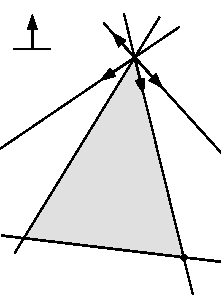
\includegraphics{part_1/chapter_4/figures/Figure1.pdf}};
		\node[right] (c) at (-1.5, 1.5) {$c$};
		\node[above] (x) at (0.5,1.7) {$x$};
		\node (y) at (1.1,-2.1) {$y$};
		\node (f) at (-0.15,1.4) {$f$};
		\node (h) at (0.35, 0.9) {$h$};
        \node (g) at (0.95, 1.3) {$g$};
        \node (-g) at (-0.3, 1.9) {$-g$};
		\node (x4=0) at (-1,1.1) {$x_4 = 0$};
		\node (x3=0) at (-1.3,-0.2) {$x_3 = 0$};
		\node (x1=0) at (-0.2,-2) {$x_1 = 0$};
		\node[right] (x2=0) at (1, -0.8) {$x_2 = 0$};
		\node[right] (x5=0) at (1, 1) {$x_5 = 0$};
	\end{tikzpicture}
	\caption{ $I_N = \braces{4,5}$ for $x$; $f$ ($x_5 > 0$) and $g$ ($x_4 >0$) are basic directions. Making $I_N = \braces{2,5}$ lead to new basic directions $h$ ($x_4 > 0$) and $-g$ ($x_2 > 0$).} \label{p1c4:fig:degenerate_basis}
\end{figure}


\section{Implementing the simplex method}

We now focus on some specific details related to alternative simplex method implementations. In a general sense, implementations of the simplex method vary in terms of how the selection of the nonbasic variables with $\overline{c}_j < 0$ that enters the basis is made. Also, the basic variable $l = \argmin_{i \in B \mid d_i <0}\braces{-x_{B(i)}/d_{B(i)}}$ to leave the basis in case of ties might be of interest, specially in the attempt of preventing cycling.

Another important aspect related to implementations of the simplex method is how matrices are represented and its consequences to memory utilisation, and how the operations related to matrix inversion are carried out. 


\subsection{Pivot or variable selection}

The rules utilised for making choices in terms of entering and leaving variables are generally referred to as \emph{pivoting rules}, though the term most commonly used to refer to the selection of nonbasic variables to enter the basis is \emph{(simplex) pricing rules}.

% TODO: add a bit more about these methods. Separate Devex and Steepest edge and give more details on both.
\begin{itemize}
	\item \emph{Greedy selection} (or Dantzig's rule): choose $x_j$, $j \in I_N$, with largest $|\overline{c}_j|$. Prone to cycling.
	\item \emph{Index-based order} (or Bland's rule): choose $x_j$,  $j \in I_N$, with smallest $j$. Prevents cycling but is computationally inefficient. 
%		\item The \alert{lexicographic} rule combines the two ideas above.
	\item \emph{Reduced cost pricing}: calculate $\overline{\theta}$ for all (or some) $j \in N$ and pick smallest $\overline{\theta}\overline{c}_j$. Calculating the actual observed change for all nonbasic variables is too computationally expensive. Partial pricing refers to the idea of only considering a subset of the nonbasic variables to calculate $\overline{\theta}\overline{c}_j$.
	\item \emph{Devex}\footnote{P. M. J. Harris (1973), Pivot Selection Methods in the Devex LP Code, Math. Prog., 57, 341--374.} and \emph{steepest-edge} \footnote{J. Forrest \& D. Goldfarb (1992), Steepest-Edge Simplex Algorithms for LP, Math. Prog., 5, 1--28.}: most commonly used by modern implementations of the simplex method available in professional-grade solvers. 
\end{itemize}


\subsection{The revised simplex method}

 
The central element in the simplex method is the calculation of the matrix $B^{-1}A_j$, from which the reduced cost vector $\overline{c}_j$, $j \in I_N$, the basic feasible direction vector $d_B$ and the step size $\overline{\theta}$ can be easily computed.

First, let us consider a more natural way of implementing the simplex method, so then we can point out how the method can be revised to be more computationally efficient. We will refer to this version as the naive simplex. The main differences between the naive and its revised version will be how $B^{-1}A_j$ is computed and the amount of information being carried over between iterations.

A somewhat natural way to implement the simplex method would be to first store in an auxiliary variable the term $p^\top = c_B^\top B^{-1}$, by solving the linear system $p^\top B = c_B^\top$. These terms have an importance on themselves, as we will see later, and they are often referred to as the ``simplex multipliers''.

Once the simplex multipliers $p$ are available, the reduced cost $c_j$ associated with the nonbasic variable index $j \in I_N$ is simply 
%
\begin{equation*}
	\overline{c}_j = c_j - p^\top A_j.	
\end{equation*}
%
Once the column $A_j$ is selected, we can then solve a second linear system $Bu = A_j$ to determine $u = B^{-1}A_j$. 

The key point that can yield computational savings is the solution of the two linear systems. As one can notice, there is a common term between the two, the inverse of the basic matrix $B^{-1}$. If this matrix can be made available at the beginning of each iteration, then the terms $c_B^\top B^{-1}$ and $B^{-1}A_j$ can be easily and more cheaply (computationally) obtained.

For that to be possible, we need an efficient manner to update the matrix $B^{-1}$ after each iteration. To see how that can be accomplished, recall that
%
\begin{align*}
	& B = [A_{B(1)}, \dots, A_{B(m)}], \text{ and } \\ 
	& \overline{B} = [A_{B(1)}, \dots, A_{B(l-1)},A_j,A_{B(l+1)}\dots, A_{B(m)}], 
\end{align*}
%
where the $l^{\text{th}}$ column $A_{B(l)}$ is precisely how the adjacent bases $B$ and $\overline{B}$ differ, with $A_j$ replacing $A_{B(l)}$ in $\overline{B}$.

We can devise an efficient manner to update $B^{-1}$ into $\overline{B}^{-1}$ utilising elementary row operations. First, let us formally define the concept.

\begin{definition}[Elementary row operations]
	Adding a constant multiple of one row to the same or another row is called an elementary row operation.
\end{definition}

Defining elementary row operations is the same of devising a matrix $Q = I + D_{ij}$ to premultiply $B$, where
%
\begin{equation*}
	D = \begin{cases}
		D_{ij} = \beta, \\
	    D_{i'j'} = 0 \text{ for all $i',j' \neq i,j$}.  
	\end{cases}
\end{equation*}
%
Calculating $QB = (I + D)B$ is the same as having the $j^{\text{th}}$ row of $B$ multiplied by a scalar $\beta$ and then having the resulting $j^{\text{th}}$ row added to the $i^{\text{th}}$ row of $B$. Before we continue, let us utilise a numerical example to clarify this procedure.
%
Let
%
\begin{equation*} 
	B = \begin{bmatrix} 1 & 2 \\ 3 & 4 \\ 5 & 6
		\end{bmatrix}
\end{equation*}
%
and suppose we would like to multiply the third row by 2 and have it then added to the first row. That means that $D_{13} = 2$ and that $Q = I + D$ would be
%
\begin{equation*} 
	Q = \begin{bmatrix} 1 & & 2\\ & 1 & \\ & & 1 	\end{bmatrix}
\end{equation*}
%
Then premultiplying $B$ by $Q$ yields
%
\begin{equation*}
	QB = \begin{bmatrix} 11 & 14 \\ 3 & 4 \\ 5 & 6
		 \end{bmatrix}.
\end{equation*}	
%
As a side notice, we have that $Q^{-1}$ exists since $\det(Q) = 1$. Furthermore, sequential elementary row operations $\braces{1,2,\dots, k}$ can be represented as $Q = Q_1Q_2,\dots Q_k$.

Going back to the purpose of updating $B^{-1}$ into $\overline{B}^{-1}$,  notice the following. Since $B^{-1}B = I$, each term $B^{-1}A_{B(i)}$ is the $i^{\text{th}}$ unit vector $e_i$ (the $i^{\text{th}}$ column of the identity matrix). That is, 
%
\begin{equation*}
	B^{-1}\overline{B} = \begin{bmatrix} \vline & & \vline & \vline & \vline & & \vline \\
		e_1 & \dots & e_{l-1} & u & e_{l+1} & \dots & e_m \\
		 \vline & & \vline & \vline & \vline & & \vline								
	\end{bmatrix} = \begin{bmatrix} 1 & & u_1 & & \\ & \ddots & \vdots &  & \\ & & u_l & & \\ & & \vdots & \ddots & \\
	& & u_m & & 1 
	 	\end{bmatrix},
\end{equation*}
%
where $u = B^{-1}A_j$. We want to define an elementary row operation matrix $Q$ such that $QB^{-1} = \overline{B}^{-1}$, or $QB^{-1}\overline{B} = I$. Therefore $Q$ will be such that the elementary row operations turn $B^{-1}\overline{B}$ into an identity matrix, i.e., that turn the vector $u$ into the unit vector $e_l$.

The main trick is that we do not need matrix multiplication to achieve it, saving considerably in computational resources. Instead, we can simply apply the elementary row operations, focusing only on the column $u$ and the operations required to turn it into the unit vector $e_l$. This can be achieved by:

\begin{enumerate}
	\item for each $i \neq l$, multiply the $l^{\text{th}}$ row by $-\frac{u_i}{u_l}$ and add to the $i^{\text{th}}$ row. This replaces $u_i$ with zero for all $i \in I \setminus \braces{l}$.
	\item Divide the $l^{\text{th}}$ row by $u_l$. This replaces $u_l$ with one.
\end{enumerate}

We can restate the simplex method in its revised form. This is presented in Algorithm \ref{p1c4:alg:revised_ximplex_method}.

\begin{algorithm}[h]
	\caption{Revised simplex method} \label{p1c4:alg:revised_ximplex_method}
	\begin{algorithmic}[1] %line numbering frequency. 
	\State {\bf initialise.} Initial basis $B$, associated BFS $x$, and $B^{-1}$ are available.
	\State Calculate $p^\top = c_B^\top B^{-1}$ and $\overline{c_j} = c_j - p^\top A_j$ for $j \in N$.
	\While {$\overline{c}_j < 0$ for some $j \in N$} \label{p1c4:alg:opt_condition} 
	    \State Choose some $j$ for which $\overline{c_j} < 0$. Calculate $u = B^{-1}A_j$. 
	    \If {$u \leq 0$} \label{p1c4:alg:unb_condition}
			\State {\bf return} $z = -\infty$.		
		\Else
			\State $\overline{\theta} = \min_{i \in I_B : u_i > 0} \braces{\frac{x_{B(i)}}{u_i}}$ and $l = \argmin_{i \in B : u_i > 0} \braces{\frac{x_{B(i)}}{u_i}}$ 
			\State Set $x_j = \overline{\theta}$ and $x_B = x - \overline{\theta}u$.
			\State Form the matrix $[B^{-1} \,|\, u]$ and perform EROs to convert it to $[\overline{B}^{-1} \, | \, e_l]$. 
			\State Make $B = B \setminus \braces{l} \cup \braces{j}$ and $B^{-1} = \overline{B}^{-1}$. 
			\State Calculate $p^\top = c_B^\top B^{-1}$ and $\overline{c}_j = c_j - p^\top A_j$ for all $j \in I_N = J \setminus I_B$.
		\EndIf
	\EndWhile
	\State {\bf return} optimal basis $B$ and optimal solution $x$.
	\end{algorithmic}
\end{algorithm}

Notice that in Algorithm \ref{p1c4:alg:revised_ximplex_method}, apart from the initialisation step, no linear systems are directly solved. Instead, elementary row operations (ERO) are performed, leading to computational savings.

The main aspect that actually make the revised simplex method ``revised'' is a matter of representation and, thus, memory allocation savings. Algorithm \ref{p1c4:alg:revised_ximplex_method} only require the maintenance of a matrix of the form 
%
\begin{equation*}
	\begin{bmatrix}
		p & | & p^\top b \\
		B^{-1} & | & u	
	\end{bmatrix}
\end{equation*}
%  
which, after each series of elementary row operations yield not only $\overline{B}^{-1}$, but also the updated simplex multipliers $\overline{p}$ and $\overline{p}^\top b = c_B^\top \overline{B}^{-1}b = c_B ^\top \overline{x}_B$, which represents the objective function value of the new basic feasible solution $\overline{x} = [\overline{x}_B, \overline{x}_N]$. This bookkeeping savings will become obvious once we discuss the tabular (or non-revised) version of the simplex method. 

Three main issues arise when considering the efficiency of implementations of the simplex method, namely, matrix (re)inversion, representation in memory, and the use of matrix decomposition strategies.
%
\begin{itemize}
	\item \emph{Reinversion:} localised updates have the side effect of accumulating truncation and round-off error. In order to correct this, solvers typically rely on periodically recalculating $B^{-1}$ which although costly, can avoid numerical issues.
	\item \emph{Representation:} A sparse representation of $Q_n = Q_1Q_2 \dots Q_{k-1}$ can be kept instead of updating $B^{-1}$. Recall that $u = \overline{B}^{-1}A_j = QB^{-1}A_j$. For larger problems, that means that a trade-off between memory allocation and the number of matrix-matrix multiplications.
	\item \emph{Decomposition:} Decomposed (e.g., LU decomposition) forms of $B$ are used to improve efficiency in storage and the solution of the linear systems to exploit the typical sparsity of linear programming problems.  	
\end{itemize}

% TODO: Improve this part, expanding on the points above.


\subsection{Tableau representation}

The tableau representation of the simplex method is useful as a concept presentation tool. It consist of a naive memory-space intensive representation of the problem elements as they are iterated between each basic feasible solution. However, it is a helpful representation under a pedagogical standpoint, and will be useful for explaining further concepts in the upcoming chapters. 

In contrast to the revised simplex method, instead of updating only $B^{-1}$, we consider the complete matrix 
%
\begin{equation*}
	B^{-1}[A ~|~ b] = \left[B^{-1}A_1, \dots, B^{-1}A_n ~|~  B^{-1}b\right].		
\end{equation*}
%
Furthermore, we adjoint a row representing the reduced cost vector $\overline{c}^\top = c^\top - c_B^\top B^{-1}A$ and the negative of the objective function value for the current basis, $ -c_Bx_B = -c_B^\top B^{-1}b$, a row often referred to as the \emph{zeroth row}. The reason why we consider the negative sign is that it allows for a simple updating rule for the zeroth row, by performing elementary row operations to make zero the $j^\text{th}$ element associated with the nonbasic variable in $B$ that becomes basic in $\overline{B}$.

The full tableau representation is given by

\begin{center}
	\begin{tabular}{ | c | c |} 
		\hline
		$c^\top - c_B^\top B^{-1}A$ & $-c_B^\top B^{-1}b$ \\ \hline
		$B^{-1}A$ & $B^{-1}b$ \\ \hline
	\end{tabular} 
	$\Rightarrow$ 
	\begin{tabular}{ | c  c  c | c |}
			\hline
			$\overline{c}_1$ & $\cdots$ & $\overline{c}_n$ & $-c_B x_B$ \\ \hline
			$\vline$ & & $\vline$ & $x_{B(1)}$ \\ 
			$B^{-1}A_1$ & $\cdots$ & $B^{-1}A_n$ & $\vdots$ \\
		    $\vline$ & & $\vline$ & $x_{B(m)}$ \\ \hline
	\end{tabular}
\end{center}
%

In this representation, we say that the $j^\text{th}$ column associated with the nonbasic variable to become basic is the \emph{pivot column} $u$. Notice that, since the tableau exposes the reduced costs $\overline{c}_j$, $j \in I_N$, it allows for trivially applying the greedy pricing strategy (by simply choosing the variables with a negative reduced cost of largest module). 

The $l^{\text{th}}$ row associated with the basic variable selected to leave the basis is the \emph{pivot row}. Again, the tableau representation facilitates the calculation of the ratios used in choosing the basic variable $l$ to leave the basis, since it amount to simply calculating the ratios between the elements on the rightmost column and those in the pivot column, disregarding those that present entries less or equal than zero and the zeroth row. The row with the minimal ratio will be that associated with the current basic variable leaving the basis. 

Once a pivot column and a pivot row have been defined, it is a matter of performing elemental row operations utilising the pivot row to turn the pivot column into the unit vector $e_l$ and turn to zero the respective zeroth element (recall that basic variables have zero reduced costs). This is the same as using elementary row operations using the pivot row to turn all elements in the pivot column zero, with exception of the \emph{pivot element} $u_l$, which is the intersection of the pivot row and the pivot column, that must be turned into one. The above highlights the main purpose of the tableau representation, which is to facilitate hand calculation.

Notice that, as we seem before, performing elementary row operations to convert the pivot column $u$ into $e_l$ converts $B^{-1}[A ~|~ b]$ into $\overline{B}^{-1}[A ~|~ b]$. Analogously, by turning the entry associated with the pivot column $u$ in the zeroth row to zero converts $[c^\top - c_B^\top B^{-1}A \mid -c_B^\top B^{-1}b]$ into $[c^\top - c_{\overline{B}}^\top \overline{B}^{-1}A \mid -c_{\overline{B}}^\top \overline{B}^{-1}b]$.

% TODO: Add a numerical example

\subsection{Generating initial feasible solutions} 

We now consider the issue of converting general linear programming problems into the standard form they are assumed to be for the simplex method. As we mentioned before, problems with constraints of the form $Ax \le b$ can be converted by simply adding nonnegative \emph{slack variables} $s \geq 0$, and trivially obtain an initial basic feasible solution (BFS) with $(x,s) = (0,b)$, with $B = I$, as
%
\begin{equation*}
		Ax \leq b \Rightarrow Ax + s = b.
\end{equation*}
%
Notice that this is equivalent to assume all original variables of the problem (i.e., those that are not slack variables) to be initialised as zero (i.e., nonbasic), since this is a trivially available initial feasible solution. However, this method does not work for constraints of the form $Ax \ge b$, as in this case, the transformation would take the form 
%
\begin{equation*}
	Ax \geq b \Rightarrow Ax - s = b \Rightarrow Ax - s + y = b.	
\end{equation*}
%
Notice that making the respective slack variable basic would yield an initial value of $-b$ (recall that $b \ge 0$ can be assumed without loss of generality), making the basic solution not feasible.

For more general problems, however, this might not be possible since simply setting the original problem variables to zero might not yield a feasible solution that can be used as a BFS. To circumvent that, we rely on \emph{artificial variables} to obtain a BFS.

Let $P : \mini\braces{c^\top x : Ax = b, x \geq 0}$, which can be achieved with appropriate transformation and assumed (without loss of generality) to have $b \geq 0$. Then, finding a BFS for $P$ amounts to finding a zero-valued optimal solution to the \emph{auxiliary problem}
%
\begin{align*}
	(AUX) : \mini &\sum_{i=1}^m y_i \\
	\st & Ax + y = b \\
	    & x,y \geq 0.	
\end{align*}
%
The auxiliary problem $AUX$ is formed by including one artificial variable for each constraint in $P$, represented by the vector $y$. Notice that the problem is represented in a somewhat compact notation, in which we assume that all slack variables used to convert inequalities into equalities have been already incorporated in the vector $x$ and matrix $A$, with the artificial variables $y$ playing the role of ``slacks'' in $AUX$ that can be assumed to be basic and trivially yield an initial BFS for $AUX$. In principle, one does not need artificial variables for the rows in which there is a positive signed slack variable (i.e., an originally less-or-equal-than constraint), but this representation allows for compactness. 

Solving $AUX$ to optimality consists of trying to find a BFS in which the value of the artificial variables are zero, since, in practice, the value of the artificial variables measures a degree of infeasibility of the current basis in the context of the original problem $P$. This means that BFS in which the artificial variable play no roles was found and that can be used as an initial BFS for solving $P$. On the other hand, if the optimal for $AUX$ is such that some of the artificial variables are nonzero, then this implies that there is no BFS for $AUX$ in which the artificial variables are all zero, or, more specifically, there is no BFS for $P$, indicating that the problem $P$ is \emph{infeasible}.

Assuming that $P$ is feasible and $\overline{y}=0$, two scenarios can arise. The first is when the optimal basis $B$ for $AUX$ is composed only by columns $A_j$ of the original matrix $A$, with no columns associated with the artificial variables. Then $B$ can be used as an initial starting basis without any issues.

The second scenario is somewhat more complicated. Often, $AUX$ is a degenerate problem and the optimal basis $B$ may contain some of the artificial variables $y$. This then requires an additional preprocessing step, which consists of the following:
%
\begin{enumerate}
	\item Let $A_{B(1)}, \dots, A_{B(k)}$ be the columns $A$ in $B$, which are linearly indepedent. Being $A$ full-rank, we can choose additional columns $A_{B(k+1)}, \dots, A_{B(m)}$ that will span $\reals^{m}$.
	\item Select the $l^{\text{th}}$ artificial variable $y_l=0$ and select a component $j$ in the $l^{\text{th}}$ row with nonzero $B^{-1}A_j$ and use elementary row operations to include $A_j$ in the basis. Repeat this $m-k$ times.
\end{enumerate}

The procedure is based on several ideas we have seem before. Since $\sum_{i=1}^m y_i$ is zero at the optimal, there must be a BFS in which the artificial variables are nonbasic (which is what (1) is referring to). Thus, step (2) can be repeated until a basis $B$ is formed including none of the artificial variables. 

Some interesting points are worth highlighting. First, notice that $B^{-1}A_{B(i)} = e_i$, $i=1, \dots, k$. Since $k < l$, the $l^{\text{th}}$ component of each of these vectors is zero, and will remain so after performing the elementary row operations. In turn, the $l^{\text{th}}$ entry of $B^{-1}A_j$ is not zero, and thus $A_j$ is linearly independent to $A_{B(1)}, \dots, A_{B(k)}$. 

However, it might be so that we find zero elements in the $l^{\text{th}}$ row. Let $g$ be the $l^{\text{th}}$ row of $B^{-1}A$ (i.e., the entries in the tableau associated with the original problem variables). If $g$ is the null vector, then $g_l$ is zero and the procedure fails. However, note that $g^\top A = 0 $ $= g^\top Ax = g^\top b$, implying that $g^\top Ax = g^\top b$ is \emph{redundant} can be removed altogether. 

This process of generating initial BFS is often referred to as \emph{Phase I} of the two-phase simplex method. Phase II consists of employing the simplex method as we developed it utilising the BFS found in the Phase I as a starting basis.


\section{Column geometry of the simplex method}

Now, let us try to develop a geometrical intuition on why it is so that the simplex method is remarkably efficient in practice. As we have seen in Theorem \ref{p1c4:thm:convergece_simplex}, althought the simplex method is guaranteed to converge, the total number of steps the algorithm might need to take before convergence grows exponentially with the number of variables and constraints, since the number of steps depends on the number of vertices of the feasible region. However, it turns out that, in practice, the simplex method typically requires $O(m)$ iterations, being one of the reasons why it has experienced tremendous success and is by far the most mature and reliable technology when it comes to optimisation. 

In order to develop a geometrical intuition on why this is the case, let us first consider an equivalently reformulated problem $P$:
%
\begin{align*}
	P : \mini & z           \\
	\st & Ax = b        \\
	& c^\top x = z      \\	
	& \sum_{j=1}^nx_j=1 \\
	& x \geq 0
\end{align*}
% 
In this reformulation, we make the objective function an auxiliary variable, so it can be easily represented on a real line, at the expense of adding an additional constraint $c^\top x = z$. Furthermore, we normalise the decision variables, so they add to one (notice that this implies a bounded feasible set). Notice that problem $P$ can be equivalently represented as  
%
\begin{align*}
	P : \mini & z     \\
	\st & x_1\begin{bmatrix}
		A_1 \\
		c_1
	\end{bmatrix} + x_2\begin{bmatrix}
		A_2 \\
		c_2
	\end{bmatrix} + \dots +
	x_n\begin{bmatrix}
		A_n \\
		c_n
	\end{bmatrix} = \begin{bmatrix}
		b \\
		z
	\end{bmatrix}\\
	& \sum_{j=1}^nx_j=1 \\
	& x \geq 0.
\end{align*}
% 
This second formulation exposes one interesting interpretation of the problem. Solving $P$ is akin to finding a set of weights $x$ that makes a convex combination (cf. Definition \ref{p1c2:def:convex_combination_hull}) of the columns of $A$ such that it constructs (or matches) $b$ in a way that the resulting combination of the respective components of the vector $c$ is minimised. Now, let us define some nomenclature that will be useful in what follows.
%
\begin{definition}[$k$-dimensional simplex] \label{p1c4:def:simplex}
	A collection of vectors $y_1, \dots, y_{k+1}$ are affinely independent if $k \leq n$ and $y_1 - y_{k+1}, \dots, y_{k} - y_{k+1}$ are linearly indepedent. The convex hull of $k+1$ affinely independent vectors is a $k$-dimensional simplex.
\end{definition}
%
Definition \ref{p1c4:def:simplex} is precisely the inspiration for the name of the simplex method. We know that only $m+1$ components of $x$ will be different than zero, since that is the number of constraints we have and, thus, the size of a basis in this case. Thus, a BFS is formed by $m+1$ $(A_i, 1)$ columns, which in turn are associated with $(A_i,c_i)$ basic points. 

Figure \ref{p1c4:fig:column_geometry} provides an illustration of the concept. In this, we have that $m=2$, so each column $A_j$ can be represented in a two-dimensional plane. Notice that a basis require three points $(A_i,c_i)$ and forms a 3-simplex. A BFS is a selection of three points $(A_i,c_i)$ such that $b$, also illustrated in the picture, can be formed by a convex combination of the $(A_i,c_i)$ forming the basis. This will be possible if $b$ happens to be inside the 3-simplex formed by these points. For example, in Figure \ref{p1c4:fig:column_geometry}, the basis formed by columns $\braces{2,3,4}$ is a BFS, while the basis $\braces{1,2,3}$ is not.

\begin{figure}[h]
	\begin{tikzpicture}
		\node (pic) at (0,0) {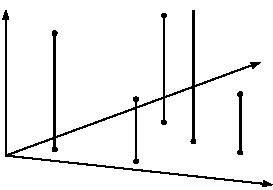
\includegraphics{part_1/chapter_4/figures/Figure2.pdf}}; 
		\node (A1) at (-1.1, -0.9) {$A_1$};
		\node (A1c1) at (-1.4, 1.3) {$(A_1, c_1)$};
		\node (A2) at (0.3, -1.1) {$A_2$};
		\node (A2c2) at (-0.4, 0.2) {$(A_2, c_2)$};
		\node (A3c3) at (0.1, 1.6) {$(A_3, c_3)$};
		\node (A3) at (0.7, -0.5) {$A_3$};
     	\node (A4) at (2, -1) {$A_4$};
		\node (A4c4) at (2.4, 0) {$(A_4, c_4)$};
     	\node (b) at (1.15, -0.8) {$b$};
    	\node (z) at (-2.4, 1.4) {$z$};    
	\end{tikzpicture}
	\caption{A solution $x$ is a convex combinations of $(A_i,c_i)$ such that $Ax= b$.} \label{p1c4:fig:column_geometry}
\end{figure}	 

We now can add a third dimension to the analysis representing the value of $z$. For that, we will use Figure \ref{p1c4:fig:column_geometry_3d}. As can be seen, each selection of basis creates a tilt in the three-dimensional simplex, such that the point $b$ is met precisely at the high corresponding to its value in the $z$ axis. This allows to compare bases according to their objective function value. And, since we are minimising, we wold like to find the basis that has its respective simplex crossing $b$ at the lowermost point.

\begin{figure}[h]
	\begin{tikzpicture}
%			\draw[help lines] (-2,-3) grid (2,3);
		\node (pic) at (0,0) {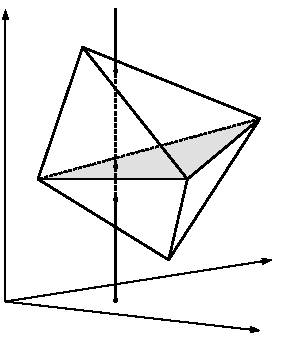
\includegraphics{part_1/chapter_4/figures/Figure3.pdf}}; 
		\node (z) at (-2.5, 2.6) {$z$};
		\node (F) at (-2, -0.1) {$F$};
		\node (G) at (-0.7, -0.5) {$G$};
        \node (H) at (-0.1, 0.1) {$H$};
        \node (I) at (-0.25, 1.55) {$I$};
		\node (B) at (-1, 2.4) {$B$};
		\node (C) at (2, 1.2) {$C$};
		\node (D) at (0.95, -0.3) {$D$};
      	\node (E) at (0.7, -1.55) {$E$};
      	\node (b) at (-0.2, -2.2) {$b$};   		   		
	\end{tikzpicture}
	\caption{A solution $x$ is a convex combinations of $(A_i,c_i)$ such that $Ax= b$.} \label{p1c4:fig:column_geometry_3d}
\end{figure}	

Notice that in Figure \ref{p1c4:fig:column_geometry_3d}, although each facet is a basic simplex, only three are feasible ($BCD$, $CDF$, and $DEF$). We can also see what one iteration of the simplex method does under this geometrical interpretation. Moving between adjacent basis means that we are replacing one vertex (say, $C$) with another (say, $E$) considering the potential for decrease in value in the $z$ axis (represented by the difference between points $H$ and $G$ onto the $z$ axis). You can also see the notion of pivoting: since we are moving between adjacent bases, two successive simplexes share an edge in common, consequently, they pivot around that edge (think about the movement of the edge $C$ moving to the point $E$ while the edge $\overline{DF}$ remains fixed).

Now we are ready to provide an insight on why the simplex method is often so efficient. The main reason is associated with the ability that the method possess of skipping bases in favour of those with most promising improvement. To see that, consider Figure \ref{p1c4:fig:column_geometry_projection}, which is a 2-dimensional schematic projection of Figure \ref{p1c4:fig:column_geometry_3d}. By using the reduced costs to guide the choice of the next basis, we tend to choose the steepest of the simplexes that can provide reductions in the objective function value, which has the side effect of allowing for skipping several basis that would have to be otherwise considered. This creates a ``sweeping effect'', in which allows the method to find optimal solutions in fewer pivots than vertices. Clearly, this can be engineered to be prevented, as there are examples purposely constructed to force the method to consider every single vertex, but the situation illustrated in Figure \ref{p1c4:fig:column_geometry_projection} is by far the most common in practice.  

% TODO: include. a discussion on dual plane, to make more concrete the relationship between the z axis and reduced costs.

\begin{figure}[h]
	\begin{tikzpicture}
%			\draw[help lines] (-2,-3) grid (2,3);
		\node (pic) at (0,0) {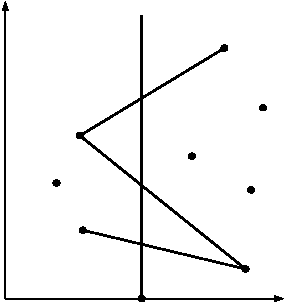
\includegraphics{part_1/chapter_4/figures/Figure4.pdf}}; 
		\node (1) at (1.8, 0.8) {$1$};
		\node (6) at (1.65, 1.8) {$6$}; 		   		
		\node (3) at (-1.3, 0.3) {$3$}; 		   		
		\node (2) at (1.1, -0.05) {$2$};
		\node (7) at (1.6, -0.6) {$7$};
		\node (4) at (-1.2, -0.5) {$4$};
		\node (8) at (-1.25, -1.3) {$8$};
		\node (5) at (2, -2) {$5$};
		\node (b) at (0, -2.7) {$b$};
	\end{tikzpicture}
	\caption{Pivots from initial basis $[A_3, A_6]$ to $[A_3, A_5]$ and to the optimal basis $[A_8, A_5]$} \label{p1c4:fig:column_geometry_projection}
\end{figure}		
 

\section{Exercises}

\subsection*{Exercise 4.1: Properties of the simplex algorithms}
Consider the simplex method applied to a standard form minimization problem, and assume that the rows of the matrix $A$ are linearly independent. For each of the statements that follow, give either a proof or a counter example.
\begin{itemize}
\item[(a)] An iteration of the simplex method might change the feasible solution while leaving the cost unchanged.
%\item[(b)] A variable that has just left the basis cannot re-enter in the very next iteration.
\item[(b)] A variable that has just entered the basis cannot leave in the very next iteration.
\item[(c)] If there is a non-degenerate optimal basis, then there exists a unique optimal basis.
%\item[(e)] If $\bf x$ is an optimal solution found by the simplex method, no more than $m$ of its components can be positive, where $m$ is the number of equality constraints.
\end{itemize}

\subsection*{Exercise 4.2: The simplex method}
Consider the problem
%
\begin{align*}
	\maxi & 40x_1 + 60 x_2   \\
	\st   & 2x_1 + x_2 \le 7 \\
		  & x_1 + x_2 \le 4  \\
		  & x_1 + 3x_2 \le 9 \\
		  & x_1, x_2 \ge 0.
\end{align*}

A feasible point for this problem is $(x_1,x_2)=(0,3)$. Formulate the problem as a minimisation problem in standard form and verify whether or not this point is optimal. If not, solve the problem by using the simplex method.

\subsection*{Exercise 4.3: Solving a tableau}
\renewcommand{\arraystretch}{1.1}
\setlength{\tabcolsep}{8pt}
Consider a linear programming problem in standard form, described in terms of the following tableau:
\[
\begin{tabular}{c|c|ccccccc}
  &   & $x_1$ & $x_2$ & $x_3$ & $x_4$ & $x_5$ & $x_6$ & $x_7$\\
\hline
  & $0$  & $0$ & $0$ & $0$ & $\delta$ & 3 & $\gamma$ & $\xi$ \\
\hline
$x_2=$   & $\beta$ & 0 & 1 & 0 & $\alpha$ & 1 & 0      &  3 \\
$x_3=$   & 2       & 0 & 0 & 1 & -2\,\,       & 2 & $\eta$ & -1\,\, \\
$x_1=$   & 3       & 1 & 0 & 0 &  0       &-1\,\, & 2      &  1
  \end{tabular}
\]
The entries $\alpha$, $\beta$, $\gamma$, $\delta$, $\eta$ and $\xi$ in the tableau are unknown parameters. Furthermore, let $\mathbf{B}$ be the basis matrix corresponding to having $x_2$, $x_3$, and $x_1$ (in that order) be the basic variables. For each one of the following statements, find the ranges of values of the various parameters that will make the statement to be true.
\begin{itemize}
\item[(a)] Phase II of the Simplex method can be applied using this as an initial tableau.
%\item[(b)] The first row in the present tableau (below the row with the reduced costs) indicates that the problem is infeasible.
\item[(b)] The corresponding basic solution is feasible, but we do not have an optimal basis.
\item[(c)] The corresponding basic solution is feasible and the first Simplex iteration indicates that the optimal cost is $-\infty$.
\item[(d)] The corresponding basic solution is feasible, $x_6$ is candidate for entering the basis, and when $x_6$ is the entering variable, $x_3$ leaves the basis.  
\item[(e)] The corresponding basic solution is feasible, $x_7$ is candidate for entering the basis, but if it does, the objective value remains unchanged.
\end{itemize}

\pagebreak

\subsection*{Exercise 4.4: Two-phase simplex method}
Solve the problem below using the two-phase simplex method. What is your conclusion about the feasibility of the problem? Verify your results by drawing the feasible region.
%
\begin{align*}
	\maxi & 5x_1 + x_2 			\\
	\st   & 2x_1 + x_2 \geq 5   \\
		  & x_2 \geq 1 			\\
		  & 2x_1 + 3x_2 \leq 12 \\
		  & x_1, x_2 \geq 0.
\end{align*}




